There are some basic mathematical and image processing principles that we need to be familiar before we start image stitching. In this chapter, we basically focus on 2D gray scale image processing and its not a big deal to extend the methods for colored images. 
\section{Image Representation}
An image consists of information and that should be represented in a form of data structure. This section discusses two main data structures used in image analysis applicable for this thesis project.
\subsection{Matrices}
In matrix representation, each pixel of the image is represented in the form of matrix. The binary images are represented by a matrix containing only zeros and ones. For N-bit gray scale images, the matrix contains the values from 0 to $2^N-1$. Figure~\ref{fig:image_matrix} shows 8-bit gray scale image in matrix form.\\

\noindent The multispectral images contain multiple matrices to represent each spectrum (e.g. RGB color images are represented by 3 matrices containing red, green and blue values). All matrix related operations (like addition, subtraction, multiplication, scaling, inverse etc.) can be applied to the images represented in matrix form. 
\begin{figure}[t]%
\begin{center}
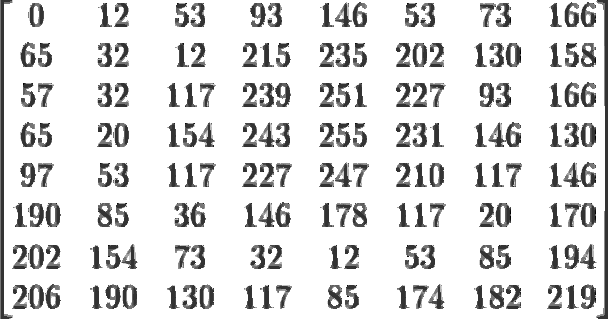
\includegraphics[width=0.6\columnwidth]{2.mainmatter/1.Introduction/figures/matrix_image}%
\caption[Image in Matrix Form]{Image represented in matrix form.The elements matrix are the pixel values}%
\label{fig:image_matrix}%
\end{center}
\end{figure}

 % Refer to Ps. 99 Sonka
\subsection{Pyramids}
\label{subsec:pyramids}
% Refer to Ps. 106
Processing higher resolution images is time consuming and are not suitable for interactive system design. So, to make it faster, we process the images in lower resolution to select the interesting parts in image and further processing is carried out to the selected parts in higher resolution~\cite{Sonka:08}.
\begin{figure}[!tb]
\begin{center}
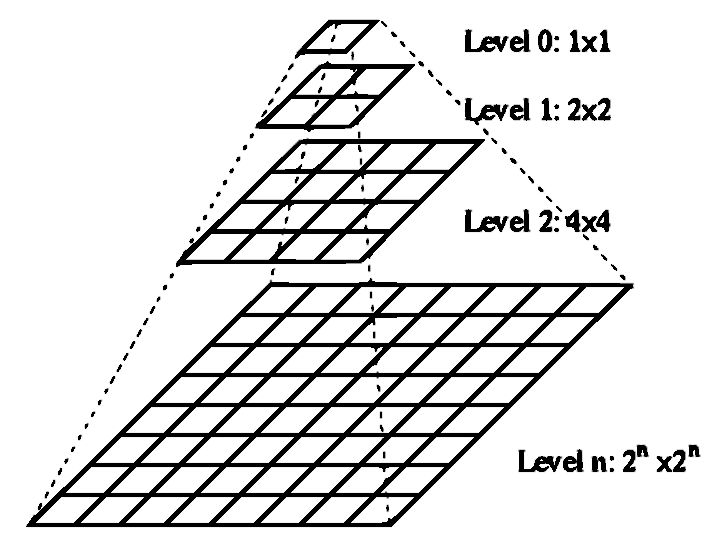
\includegraphics[width=1\textwidth]{2.mainmatter/1.Introduction/figures/Image_Pyramid}%
\caption[Image Pyramids]{Image Pyramids. \imgsrc{(Image source: http://fourier.eng.hmc.edu)}}%
\label{fig:pyramids}%
\end{center}
\end{figure}
This is achieved by generating matrix pyramids of an image which consists of a sequence of images $\{M_L,M_{L-1},...,M_0\}$ (figure~\ref{fig:pyramids}) where $M_L$ has the same dimension and elements as the original image and $M_{i-1}$  will have half resolution of $M_i$. We can create image up to $M_0$ (i.e. 1 pixel) if we have square image with dimension multiple of 2. Generally, we will select a level and generate the pyramid of images up to that level. The level to be selected depends upon the specific problem.\\

\noindent There are two types of pyramids: low-pass pyramids and band-pass pyramids. In low pass pyramid, we smooth the image with appropriate smoothing filter, and sub sample the smoothed image to create smaller image.\footnote{Gaussian pyramid is created using Gaussian smoothing filter. If we go from bottom to top, in each level, the image size is reduced by $\frac{1}{2}$} Band pass pyramid, on the other hand, is obtained by creating the difference between the adjacent levels in the pyramid. To compute pixel-wise differences, the size of the images should be same, so, we have to implement some interpolation or scaling techniques.


\section{Brightness Transformation}
Brightness transformation is carried out to make the images look more clearer. In brightness transformation, the intensity of the image pixels are changed using one of the following methods:
%Brightness Thresholding
\begin{description}
\item[Brightness Thresholding]
We select an intensity value P and then the image pixels with intensity less than p are set to zero and other pixels are set to 1 resulting black-and-white image. 

\item[Histogram Equalization]
Histogram equalization is used to enhance contrast by creating an image with equally distributed brightness levels over the whole brightness scale. If an image consists of pixels with limited level of intensities, then the histogram equalization assigns all range of intensities to the pixels which results increase in contrast. For algorithm, please refer to the book by Sonka \textit{et al}~\cite{Sonka:08}.

\begin{figure}%
\centering
\subfloat[]{%

\includegraphics[width=0.3\columnwidth]{2.mainmatter/1.Introduction/figures/gray_scale_original}%
\label{fig:gray_image}%
}%
\hspace{8pt}%
\subfloat[]{%

\includegraphics[width=0.3\columnwidth]{2.mainmatter/1.Introduction/figures/gray_scale_equalized.pdf}%
\label{fig:hist_trans_image}%
}%
\caption[Histogram Transformation]{Histogram Transformation:
	\subref{fig:gray_image} is original image;
	\subref{fig:hist_trans_image} is histogram transformed image.}%
\label{fig:hist_trans}%
\end{figure}

%\subsection*{Logarithmic Gray-scale Transformation}


\item[Look-up Table Transformation]
Look-up table is used to transform brightness in real time. The transformation information of all possible gray levels is stored in look-up table, and the transformation is carried out using the table. For example, 8 bit image contains 256 gray levels and only 256 bytes of memory is required for look-up table. 
\item[Pseudo-color Transformation]
The brightness of the pixels are represented by some color value to perceive more detail information. Also human eye is more sensitive to color change than brightness change. 
\end{description}

\section{Geometric Transformation}
In geometric transformation, we use a vector function \emph{T} which maps the pixel (x,y) to a new position (x',y') defined by the following two component equations:
\begin{equation}
x'=T_x(x,y), y'=T_y(x,y)
\label{eq:geom-trans}
\end{equation}
The transformation vector function \textbf{T} known in advance or sometimes we calculate from original and transformed images by matching of the corresponding pixels. 

\subsection*{Pixel Co-ordinate Transformation}
The co-ordinates of the input image pixels are mapped to the point in the output image. The geometric transform can be classified as
\begin{itemize}
	%\item {\textit{Bilinear Transform}} The bilinear transform is represented by:
	%\begin{equation}
	%\begin{array}{lcl}
	%x' & = & a_0+a_1x+a_2y+a_3xy,\\	
	%y' & = & b_0+b_1x+b_2y+b_3xy
	%	\end{array}	
	%\label{eq:bilinear-trans}
	%\end{equation}
	%For bilinear transform, we need four pairs of corresponding points.
	
	\item {\textit{Affine Transform}}
	The affine transform is simple and only 3 pairs of corresponding points are sufficient to find the coefficients.
	\begin{equation}
	\begin{array}{lcl}
		x' & = & a_0+a_1x+a_2y,\\
		y' & = & b_0+ b_1x+ b_2y
	\end{array}
	\label{eq:affine-trans}
	\end{equation}
	The affine transform consists of rotation, translation, scaling and skewing. 
	
	\item {\textit{Perspective Transform}}
	The perspective transform also called \emph{homography} denoted by a 3 x 3 matrix \textit{H} and the transformation is carried out as:
	\begin{equation}	
		x'  =  \frac{h_{00}x+h_{01}y+h_{02}}{h_{20}x+h_{21}y+h_{22}} \mbox{ and } 
		y'  =  \frac{h_{10}x+h_{11}y+h_{12}}{h_{20}x+h_{21}y+h_{22}}	
	\label{eq:perspective-transform}
	\end{equation}
	The perspective transforms preserve straight lines and are appropriate for 3D scenes observed under pure camera rotation or planes observed under general 3D motion~\cite{Szeliski:06}. We need four pairs of corresponding points for perspective transform.
	
	%\begin{figure}%
	%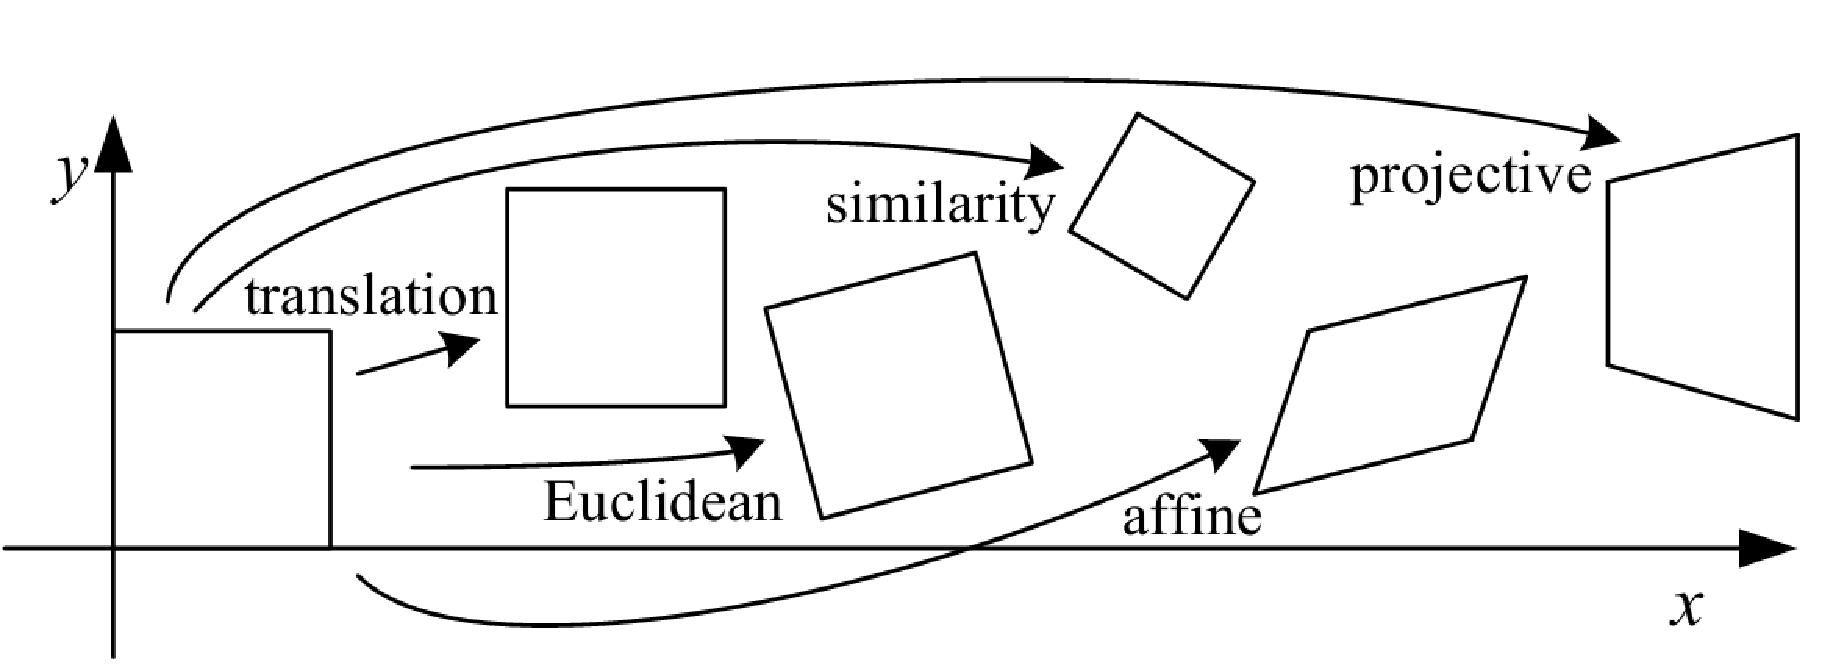
\includegraphics[width=\columnwidth]{2.mainmatter/1.Introduction/figures/2D-planar-transformation}%
	%\caption[Basic 2D Planar Transformation]{Basic 2D planar transformation. Image source:\cite{Szeliski:06}}%
	%\label{}%
	%\end{figure}
	
\end{itemize}

\subsection*{Brightness Interpolation}
The transformation generally results the continuous co-ordinate values (real numbers). The intensity value of specific integer grid in the output image is set by interpolating the brightness of neighboring non-integer samples. Brightness interpolation influences image quality. The simpler the interpolation, the greater is the loss in geometric influences and photometric accuracy~\cite{Sonka:08}. The most common interpolation methods are \emph{nearest neighbor}, \emph{linear} and \emph{bi-cubic}.

\section{Image Smoothing}
\label{sec:image-smoothing}
% Refer ps. 125
If an image contains a lot of noise, we need to have proper mechanism to reduce the noise using image smoothing methods. Generally, smoothing methods blur the edge information, so if we need to preserve the edge information, then we have to implement ``\textit{edge preserving}'' image smoothing methods. 
\subsection*{Averaging}
The noise present in the image at each pixel is an independent random value with zero mean and standard deviation $\sigma$. So, if we could get n images of the same static scene, we estimate the average of the images to remove out the noise. It is to be noted that for averaging, we need more than one images of the same scene.

\subsection*{Median Filter}
The median filter is very effective noise reduction technique because if we use it appropriately, it can reduce the noise while preserving the edge information~\cite{Donoho:09}. The median value is chosen from the pixels defined by kernel window, and since this process is carried out all the pixels in the image, it is slower method for high resolution image. Median filter is very widely used in digital image processing to remove \emph{speckle noise} and \emph{salt \& pepper noise}.  

\subsection*{Gaussian Filter}
In Gaussian filter, the image is convolved with the Gaussian function to reduce image noise. In digital image processing, a kernel window defines the effective neighborhood pixels. So, larger window size creates more blurred image. Fourier transform of a Gaussian function is another Gaussian, so Gaussian blur has the effect of reducing the high frequency components (i.e. low pass filter). \\
\begin{equation}
L(x,y,\sigma)=G(x,y,\sigma)* I(x,y)
\label{eq:gaussian_blur}
\end{equation}
where * is the convolution operation in $x$ and $y$, and 
\begin{equation}
G(x,y,\sigma)=\frac{1}{2 \pi \sigma^2} e^{-\frac{(x^2+y^2)}{2 \sigma^2}}
\label{eq:gaussian-function}
\end{equation}

\noindent Apart from smoothing, Gaussian filter can be used to generate different scales of an image as a processing stage in computer vision algorithms. For higher resolution images, the processing on original images might be complicated, so lower resolution scaled image is used for simplicity (section~\ref{subsec:pyramids}).\\

\noindent The derivative based edge detectors are sensitive to noise, so Gaussian blur filter is commonly used before the edge detection algorithm is carried out. This is called \emph{Laplacian of Gaussian} or \emph{LoG} filtering.

\section{Edge Detection}
\label{sec:edge-detection}
The edge detectors are very important in computer vision which helps for image understanding and perception by finding lines, region boundaries etc. Edges are detected by identifying the intensity changes in the image; edges are the pixels in the image where intensity changes abruptly. Edge detection is opposite to smoothing; in smoothing we remove high frequency components while in edge detection, we remove low frequency component in the image. \\

\noindent Edge detection is not a trivial task; we can not create a general edge detector working for all types of images. Generally, edge detectors work approximating the derivative (first or second order) of the image function. There are some operators such as \textit{Roberts}, \textit{Sobel}, \textit{Prewitt}, etc. which approximate the first order x- and y- derivatives of the image and calculate the resulting magnitude and direction of the edges. The alternative methods of edge detection use second derivative of the image function and the edge pixels will be the zero crossings of the second derivative.\\

\noindent The above mentioned derivative based methods are very sensitive to the noise in the image~\cite{ziou:98}~\cite{lindegerg:96}. So, we have to implement some noise reduction mechanism before differentiation of image is carried out. 

\subsection{Laplacian of Gaussian}
Before we compute the image derivative, we convolve the image with Gaussian filter to suppress the noise present in the image. Suppose, $f(x,y)$ be image function, $G_\sigma(x,y)$ be the Gaussian kernel of width $\sigma$, then
\begin{equation}
\Delta [G_\sigma(x,y) \otimes f(x,y)]=[\Delta G_\sigma(x,y)] \otimes f(x,y) = LoG \otimes f(x,y)\\
\label{eq:LoG1}
\end{equation}
where
\begin{equation}
LoG=\frac{x^2+y^2-2\sigma^2}{\sigma^4}e^{\frac{-(x^2+y^2)}{2\sigma^2}}
\label{eq:LoG2}
\end{equation}

\noindent Thus, from above equation, we conclude that Laplacian operator to the Gaussian smoothed image is equivalent to applying \emph{Laplacian of Gaussian (LoG)} operator to the original image. 

\subsection{Approximation with Difference of Gaussian}
The Laplacian of Gaussian (LoG) can be efficiently implemented using \emph{Difference of Gaussian (DoG)} at different scales. Suppose we used Gaussian kernels $G_{\sigma1}$ and $G_{\sigma2}$ to get smoothed images $g_{\sigma1}(x,y)$ and $g_{\sigma2}(x,y)$, then
\begin{equation}
g_{\sigma1}(x,y)-g_{\sigma2}(x,y)= (G_{\sigma1}-G_{\sigma2}) \otimes f(x,y)=DoG \otimes f(x,y)
\label{eq:DoG}
\end{equation}
\begin{figure}%
\centering
\includegraphics[width=1.0\columnwidth]{2.mainmatter/1.Introduction/figures/DoG-Log}%
\caption[Comparison of DoG and LoG]{Comparison of DoG and LoG. \newline \quad \imgsrc{(Image source: http://en.wikipedia.org/wiki/Difference\_of\_Gaussian)}}%
\label{fig:DoG-LoG}%
\end{figure}
\noindent The comparison graph in figure~\ref{fig:DoG-LoG} shows the similarity between DoG and LoG operators. Thus, we can approximate Laplacian of Gaussian by simply subtracting the Gaussian blurred images in different scales. 

\section{Error Metrics}
Error metrics give the measurement of similarity between two images. So, in registration process, we try to align the two images that gives optimal error value. The direct methods of image matching choose a suitable error metrics to compare the images~\cite{Szeliski:06} and the search process will try to get the optimal error value. 
\subsection*{Sum of Squared Differences}
The sum of squared differences (SSD) gives the dissimilarity measurement between two images. So, in alignment process, we try to minimize the SSD value which is calculated as follows:
\begin{equation}
E_{SSD}=\sum_{i}{[I_1(x_i)-I_0(x_i)]^2}=\sum_{i}{e_i^2}
\label{eq:ssd}
\end{equation}
where $e_i=I_1(x_i)-I_0(x_i)$ is \emph{residual error}.

\subsection*{Correlation}
The cross-correlation of the two aligned images are calculated,
\begin{equation}
E_{CC}=\sum_{i}{I_0(x_i)I_1(x_i)}
\label{eq:cross-cor}
\end{equation}
The cross-correlation value between two images does not give accurate result in case when a very bright patch exists in one of the images~\cite{Szeliski:06}. So, \emph{Normalized Cross-Correlation} (NCC) is commonly used,
\begin{equation}
E_{NCC}=\frac{\sum_{i}{[I_0(x_i)-\overline{I_0}] [I_1(x_i)-\overline{I_1}]}}{\sqrt{\sum_{i}{[I_0(x_i)-\overline{I_0}]^2[I_1(x_i)-\overline{I_1}]^2}}}
\label{eq:}
\end{equation}
where 
\begin{equation}
\overline{I_0}=\frac{1}{N}\sum_{i}{I_0(x_i)}  
\label{eq:}
\end{equation}

\begin{equation}
\overline{I_1}=\frac{1}{N}\sum_{i}{I_1(x_i)}
\label{eq:}
\end{equation}
The NCC value 1 indicates the two images are exactly same. To get the best alignment, we transform the image in such a way that it gives maximum NCC value.

\subsection*{Key Points Matching}
The key-points (feature points) between the images are identified by using some key-point detectors. We implement matching algorithm to get the matching points. The points which do not get any matching point are counted for both the images to measure the dissimilarity between the images. For perfectly matching images, the count will be zero implies the images are same. The larger the number of count, the more dissimilarity between the images.

\section{Corners in Image}
\label{sec:corners-in-image}
%Refer Sonka 157 and others
The geometric transformation parameters are estimated using the position of corresponding points. The same transformation generally hold for almost all pixels of the image and the necessary number of corresponding pairs of points is usually rather small and is equal to the number of parameters of the transformation. The same transformation usually holds for almost all pixels of the image. We have to examine all possible pairs of pixels to find out the correspondence and this is computationally expensive. If two images have n pixels each,the complexity is O($n^2$). So, to simplify this problem, we find out the \emph{interest points (corners)} and those interest points are used to find out correspondences for estimation of transformation parameters. The corner in the image can be defined as a pixel in its small neighborhood where there are two dominant and different edge directions\cite{Sonka:08}. The number of interest points are much smaller than the pixels in the image, so it greatly reduces the computational complexity.\\

\noindent The corner detectors generally use the gray scale image as input and do some processing and the final result is an image with pixel values proportional to the likelihood of the corner and we use thresholds to find out the corner points. We can get the required number of interest points by using proper threshold. Corner detectors are not usually very robust. To overcome this problem, larger number of corners are detected than needed for estimating accurate transformation. This is achieved by decreasing the threshold value. We must be careful it should not be too less; otherwise it might get very large number of corners which makes the further processing very slow. The threshold value is specific to the type and property of the image for example, the image which contains a lot of variations, larger threshold value is capable of giving sufficient number of corners while image containing plain regions might need smaller threshold value.

\subsection{Requirements of a Corner Detector}
\label{sec:req-corner-detector}
Parks \textit{et al}~\cite{Parks:11} defines some criteria for a corner detector:
\begin{itemize}
	\item All ``true corners'' should be detected.
	\item No ``false corners'' should be detected. 
	\item Corner points should be well localized.
  \item Detector should have a high repeatability rate (good stability).
	\item Detector should be robust with respect to noise.
	\item Detector should be computationally efficient.	
\end{itemize}

\subsection{Corner Detection}
This section  describes the general steps for corner detection. The following basic steps (flowchart in figure~\ref{fig:flowchart_corner-detection}) are carried out by corner detectors:
\begin{description}
\item [\textit{i. Apply Corner Operator:}] Gray scale image is as input and for each pixel, the corner operator is applied to get the \textit{cornerness measure} of the pixel~\cite{Parks:11}. Generally, a small window centered on a pixel is used to measure the cornerness of the pixel. The output of this step is \textit{cornerness map} and it has the same dimension as the input image.

\begin{figure}[H]%
\centering
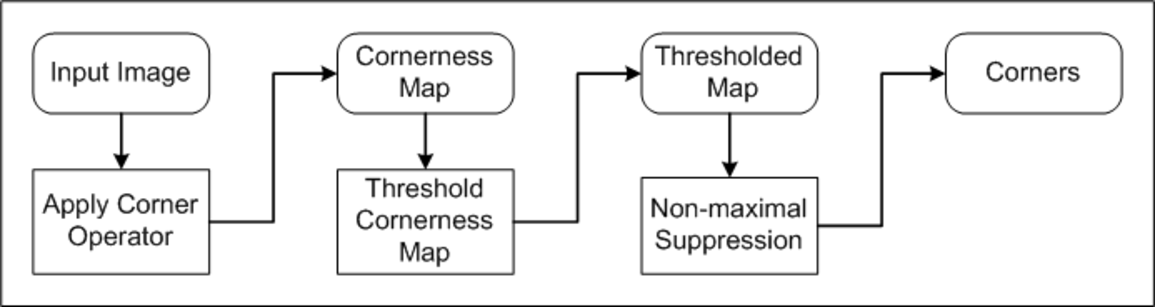
\includegraphics[width=1\columnwidth]{2.mainmatter/1.Introduction/figures/CornerFlowChart}%
\caption[Flowchart for Corner Detectors]{Flowchart for corner detectors.}%
\label{fig:flowchart_corner-detection}%
\end{figure}


\item [\textit{ii. Threshold Cornerness Map:}] The cornerness map is now thresholded to remove the false corners. We set a threshold value that will be able retain true corners.\footnote{Generally, there is no threshold value that can remove all false corner while retaining all true corners. So, the appropriate threshold is dependent on application requirements.}. There is no straightforward method to choose the threshold value, it is application dependent and requires trial and error experimentation~\cite{Parks:11}.
\item [\textit{iii. Non-maximal Suppression:}] The non-maximal suppression is carried out to get the local maxima of the thresholded cornerness map. A distance value is chosen and cornerness measure of all the pixels within the distance will be zero except the largest one. Then the result is cornerness map with non-zero points as corners. 
\end{description}

%Include the theories and basic principles required for image stitching
